
% --- SLIDE 5: WHERE THE DATA LIVES ---
\begin{frame}{Where Does the Tracking Data Actually Live?}

    \centering
    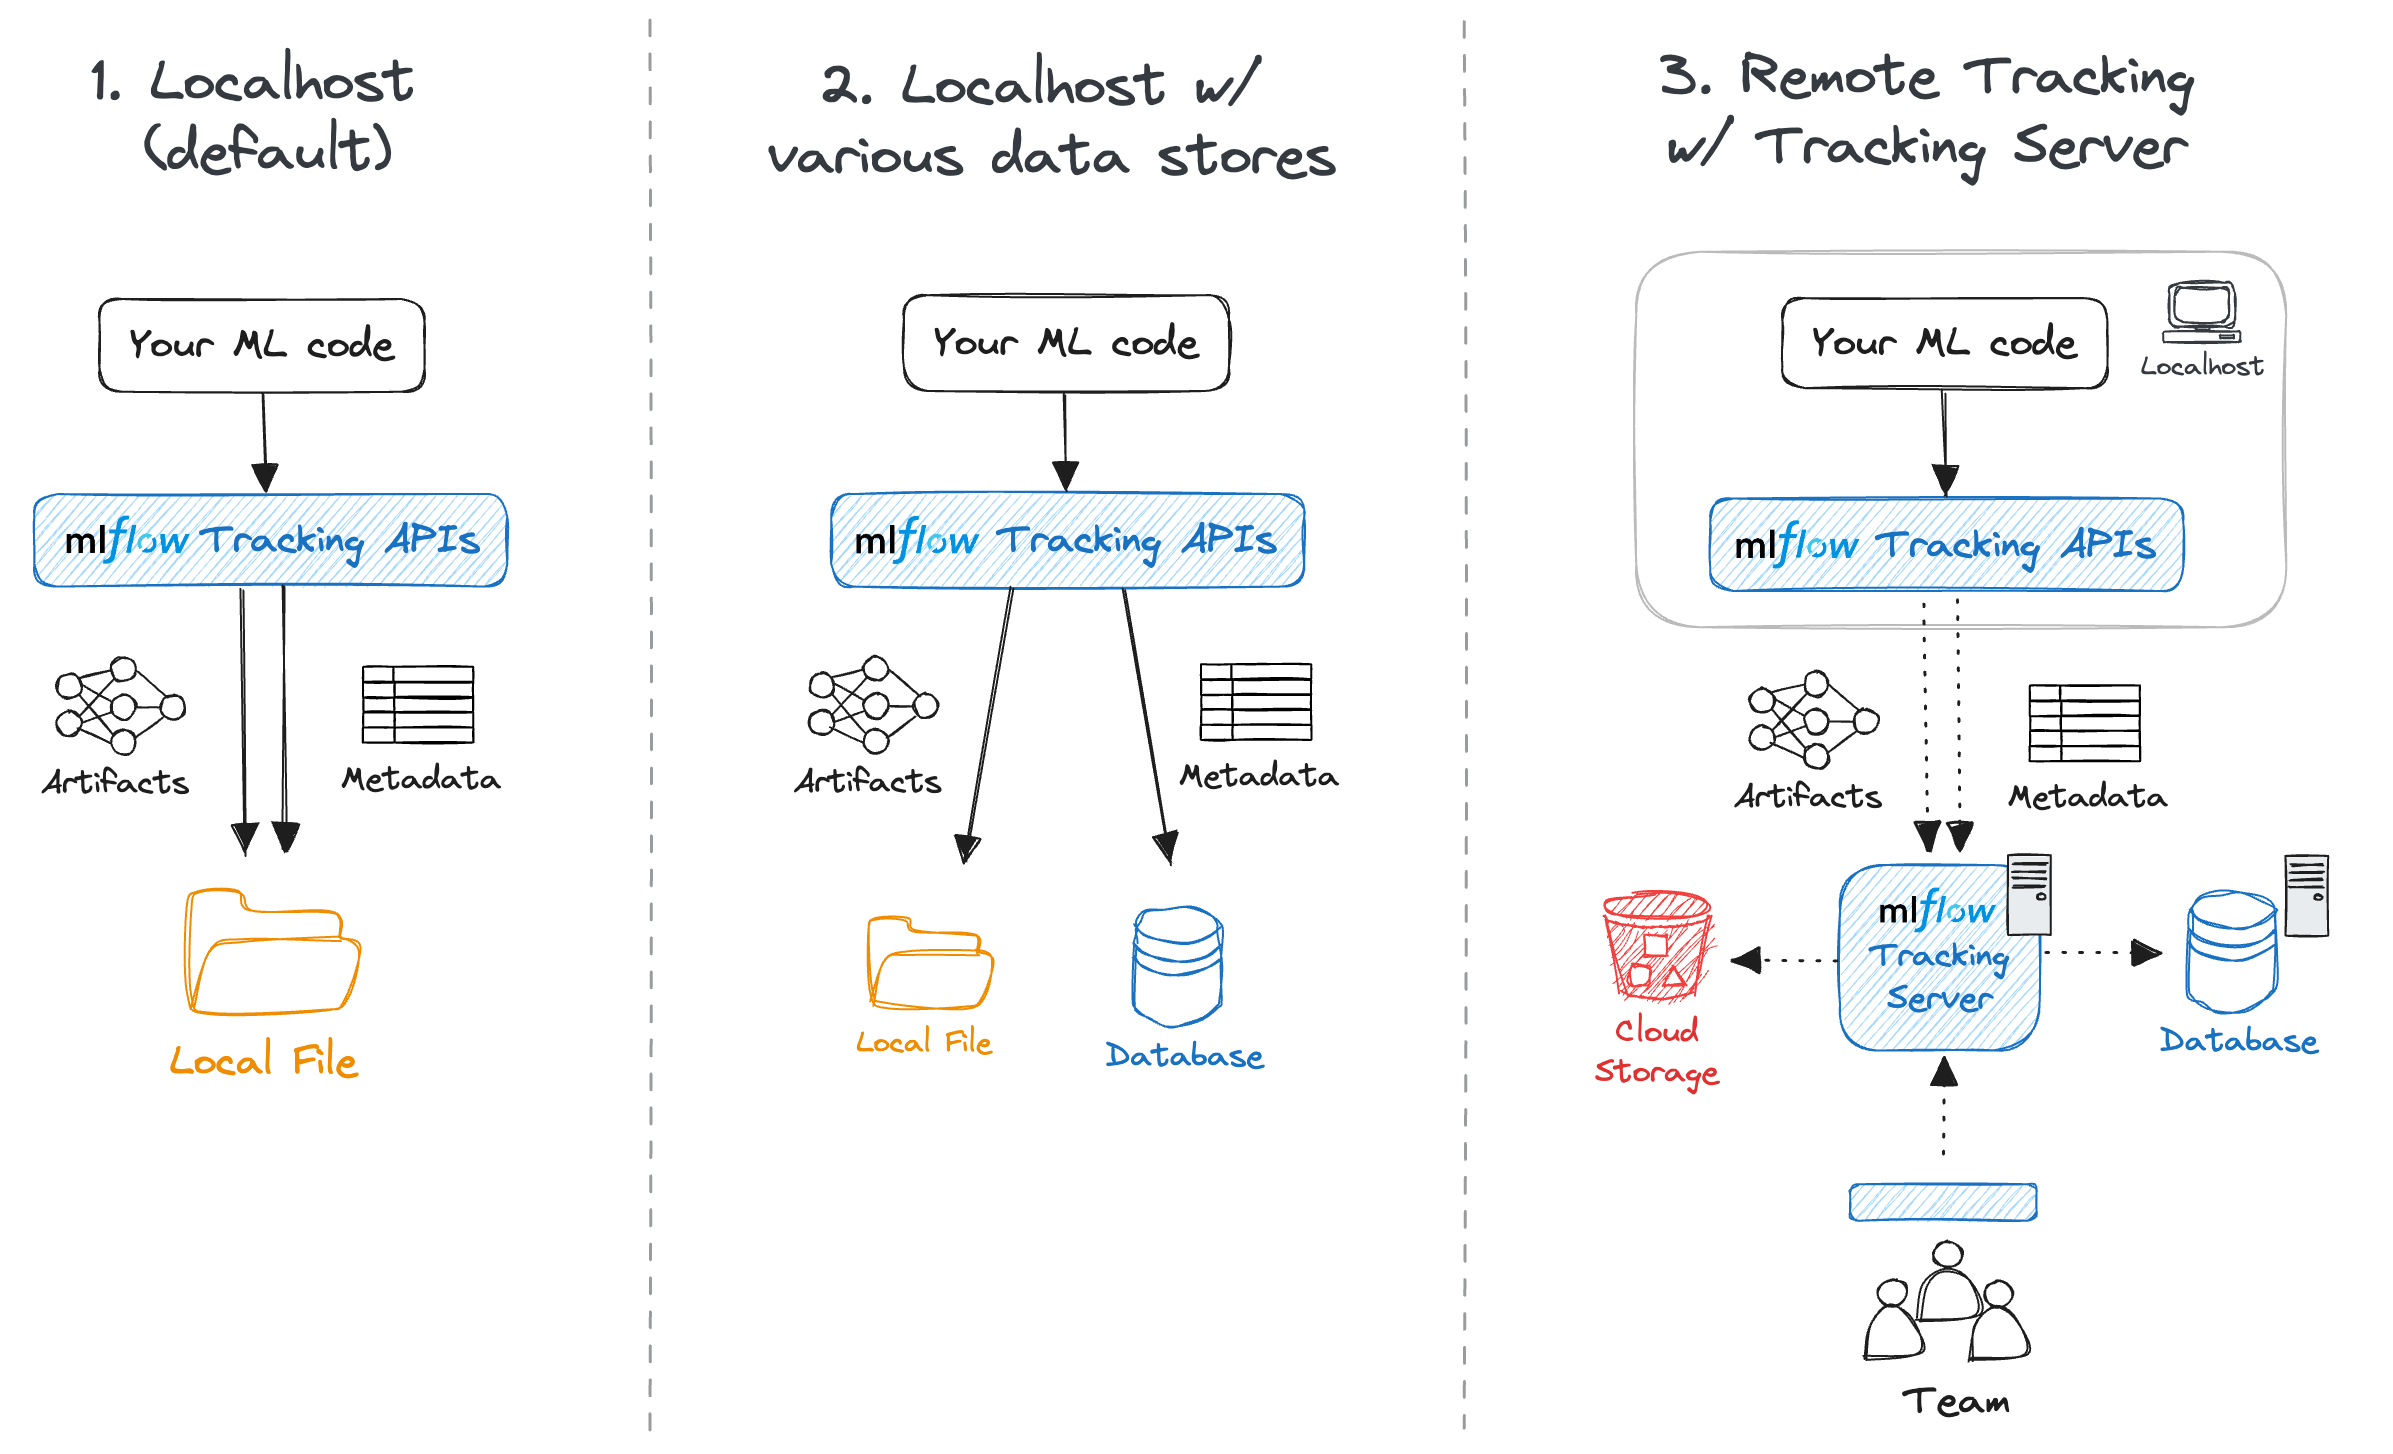
\includegraphics[width=0.86\textwidth,height=0.42\textheight,keepaspectratio]{images/mlops-foundations/mlflow_tracking_setup_overview.png}

    {\scriptsize Source: MLflow documentation, ``MLflow Tracking,''
    \href{https://mlflow.org/docs/latest/ml/tracking/}{mlflow.org/docs/latest/ml/tracking}.}

    \vspace{0.5em}
    \begin{itemize}
        \small
        \item \textbf{Metadata} (params, metrics, tags) goes to a database; \textbf{artifacts} (model files,
              plots) go to object storage. They are separate stores for a reason: one is small and queried,
              the other is large and streamed.
        \item Solo work: local files, zero setup. Team work: one shared tracking server, so ``my numbers''
              and ``your numbers'' live in the same place.
    \end{itemize}

\end{frame}
